\documentclass{article} % For LaTeX2e
\usepackage{nips15submit_e,times}
\usepackage{hyperref}
\usepackage{graphicx}
\usepackage{url}
\usepackage{amsmath}
%\documentstyle[nips14submit_09,times,art10]{article} % For LaTeX 2.09
\newcommand\BibTeX{B{\sc ib}\TeX}

\title{LSTM for Sentiment Analysis on Twitter}

\author{
Trapit Bansal
\And
Kate Silverstein
\And
Jun Wang
}

%% \author{
%% David S.~Hippocampus\thanks{ Use footnote for providing further information
%% about author (webpage, alternative address)---\emph{not} for acknowledging
%% funding agencies.} \\
%% Department of Computer Science\\
%% Cranberry-Lemon University\\
%% Pittsburgh, PA 15213 \\
%% \texttt{hippo@cs.cranberry-lemon.edu} \\
%% \And
%% Coauthor \\
%% Affiliation \\
%% Address \\
%% \texttt{email} \\
%% \AND
%% Coauthor \\
%% Affiliation \\
%% Address \\
%% \texttt{email} \\
%% \And
%% Coauthor \\
%% Affiliation \\
%% Address \\
%% \texttt{email} \\
%% \And
%% Coauthor \\
%% Affiliation \\
%% Address \\
%% \texttt{email} \\
%% (if needed)\\
%% }


% The \author macro works with any number of authors. There are two commands
% used to separate the names and addresses of multiple authors: \And and \AND.
%
% Using \And between authors leaves it to \LaTeX{} to determine where to break
% the lines. Using \AND forces a linebreak at that point. So, if \LaTeX{}
% puts 3 of 4 authors names on the first line, and the last on the second
% line, try using \AND instead of \And before the third author name.

\newcommand{\fix}{\marginpar{FIX}}
\newcommand{\new}{\marginpar{NEW}}

\nipsfinalcopy % Uncomment for camera-ready version

\begin{document}


\maketitle

\begin{abstract}
We show promising empirical evidence that character-level LSTMs perform well for sentiment analysis on tweets, which are ``noisy'', in that users think of millions of new words and spellings of words every day, and ``brief'', in that they are constrained to $140$ characters. This type of text data is becoming an important research focus in the field of NLP, as data is often cheap to collect in high volume and can provide important insight into society-wide trends. Our model achieves $84 \%$ accuracy, a result competitive with the state of the art for binary sentiment classification on tweets.
\end{abstract}

\section{Introduction}
% why analysis sentiment expecially twitter
In the last few years, microblogging has become a very popular communication tool in people's social life.
On microblogging platforms, such as Twitter\footnote{\url{https://twitter.com/}} and Facebook\footnote{\url{https://www.facebook.com/}}, a diverse range of people are attracted to post short sentences, images, and video links to share life issues and opinions.
This popularity results in enormous amount of information covering a wide range of topics on the brands, products, politics and social events. 
Such data is a valuable and efficient source for marketing and social studies. 
Sentiment analysis on microblogging has obtained special interest, because it determines the attitude of a user with respect to some topic or product and thus provides provide convincing information
For example, it may help manufacturing companies to know how people like their product (or service), what would people prefer.  

In this paper, we focus on using sentiment analysis on Twitter. 
Twitter is an extremely popular microblogging platform which allows people to post messages of up to 140 characters.
Because of the short nature of tweets, people often post twitter messages (called Tweets) frequently while attending events like product launches, movie premiers, music concerts or just to express their opinion on a trending or current topic.
As such, they can be a valuable source of public opinion or feedback \cite{o2010tweets, bollen2011twitter, bollen2009modeling}.
Realizing this importance, analyzing sentiment of Tweets has been a recurring task in the SemEval \footnote{\url{http://alt.qcri.org/semeval2016/task4/}} competitions.

%We restrict our interest on Twitter for the following reasons: 
%People are posting on various topics on Twitter, thus it is a valuable source of data; Twitter is one of the most popular microblogging platform and the number of messages are growing everyday. The collected corpus can be arbitrary large. Users of Twitter have various background and have different language conventions. It is possible to collect tweets of wide diversity in both topics and language models.

Although there exists plenty of work on text classification, some unique characteristics of tweets present special challenges for sentiment analysis:
1) Tweets are short in length. There is a limitation of $140$ words for each tweet which makes analyzing them challenging \cite{mehrotra2013improving}; 2) The language used in tweets is very informal with misspellings (often intentional, like different spellings of "cool": coool, coolll, coooolll!!), new words, slangs, and URLs;
3) The number of tweets increases at a very fast pace, and with new data comes new words, new trends in using abbreviations, which lead to a frequent problem of out-of-vocabulary words
4) Special symbols and their combinations are often used, like emoticons and hashtags.

% what we did
Keeping in view the challenges posed by the nature of tweets, 
in this paper, we propose to use bi-directional Long Short-Term Memory (LSTM) 
networks which operate at {\it character-level input} and make predictions at the tweet-level. Such networks naturally handle the problem of very large vocabulary sizes and the presence of sub-word information, without having to keep many trained embedding which would result from keeping very large vocabularies.
We find that the model interestingly performs {\bf better} than equivalent LSTM model which operates at the word level (even when initialized with a variety of pre-trained embeddings).
We also compare our results with Dynamic Convolutional Neural Network (DCNN) \cite{kalchbrenner2014convolutional} which has shown state of the art performance on Twitter sentiment classification \cite{severynunitn}.
We explore the properties of the character LSTM model and find that it learns to find meaning in composition of characters and can effectively relate sub-word information (like presence of multiple exclamation marks) to the sentiment of the tweet.


%We train our model on $1.6$ M distantly-supervised tweets collected by Go et. al. \cite{go2009twitter}, and evaluate the results on SemEval-2016 Task 4. Currently we focus on polarity classification, and plan to apply our model on 5-point scale classification in the future. 

% the structure of the paper
This paper is laid out as follows: in Section 2, we describe prior work on sentiment classification using deep learning. In Section 3, we describe the structure of our model. In Section 4, we describe the datasets used to train and evaluate our model, as well as results from several experiments. We conclude with an analysis of our results, as well as describe areas of future research.


\section{Related Work}
Twitter sentiment analysis is increasingly drawing attention of researchers in recent years. 
Given the length limitations on tweets, sentiment analysis of tweets is often considered similar to sentence-level sentiment analysis \cite{kouloumpis2011twitter}.
However, phrase and sentence level approaches can hardly define the sentiment of some specific topics. Considering opinions adhering on different topics, Wang et. al. \cite{wang2011topic} proposed a hashtag-level sentiment classification method  to generate the overall sentiment polarity for a given hashtag.
Recently, following the work of \cite{mikolov2013efficient} some researchers used neural network to implement sentiment classification. 
For example, Kim \cite{kim2014convolutional} adopted convolutional neural networks to learn sentiment-bearing sentence vectors, Mikolov et al. \cite{mikolov2013distributed} proposed Paragraph vector which outperformed bag-of-words model for sentiment analysis, and Tang et. al. \cite{tang2014learning} used ConvNets to learn sentiment specific word embedding (SSWE), which encodes sentiment information in the continuous
representation of words.
Furthermore, Kalchbrenner \cite{kalchbrenner2014convolutional} proposed a Dynamic Convolutional Neural Network (DCNN) which uses dynamic k-max pooling, a global pooling operation over linear sequences.
Instead of directly applying ConvNets to embeddings of words, \cite{zhang2015character} applies the network only on characters. They showed that the deep ConvNets does not require knowledge of words and thus can work for different languages.
LSTM \cite{hochreiter1997long} is another state-of-the-art semantic composition models for sentiment classification \cite{li2015tree}. Similar to DCNN, it also learns fixed-length vectors for sentences of varying length, captures words order in a sentence and does not depend on external dependency or constituency parse results.

\subsection{Dynamic Convolutional Neural Networks (DCNN)}
We briefly review the architecture of DCNN \cite{kalchbrenner2014convolutional} which has shown state of the art performance for sentiment classification on Twitter. The winning entry for SemEval15 \cite{severynunitn} task on Twitter sentiment classification also used DCNN. Figure \ref{fig:dcnn} summarizes the architecture.

When used for sentiment classification on Twitter, the input to the DCNN is a matrix of word embeddings for each word in the tweet. For example, if the tweet consists of $s$ words then the input to the DCCNN is:
\begin{flalign*}
	S = 
	\begin{bmatrix}
	| & | & \ldots & | \\
	w_1 & w_2 & \ldots & w_s \\
	| & | & \ldots & | \\
	\end{bmatrix}_{k\times s}
\end{flalign*}
where each $w_i \in R^k$ is a $k$-dimensional dense word embedding \cite{mikolov2013distributed}.
The architecture consists of multiple layers of convolutions and max-pooling on top of the input matrix, followed a fully connected layer which is input to a softmax. The convolutions are of type \emph{wide-convolutions} of one-dimension. For example, for the input matrix $S \in R^{k\times s}$, a wide-convolution filter operating on $S$ will consist of convolution weights $m\in R^{k\times c}$ and will result in a matrix having dimension $k \times (s+c-1)$. Note here $c$ is the convolution filter width, which is a hyperparameter.
The max-pooling operations presented in \cite{kalchbrenner2014convolutional} are different from the regular max-pooling. They present {\it dynamic $k$-max pooling}. $k$-max pooling takes the top $k$ maximum activations as opposed to just the maximum activation and the value of $k$ is selected dynamically based on the following formula: $k_l = \max \left( k_{top}, 	\lceil \frac{L-l}{L} s\rceil \right)$, where $l$ is number of current convolution layer, $L$ is total number of convolutions and $k_{top}$ is a fixed hyperparameter. 
Note that while \cite{kalchbrenner2014convolutional} used multiple layers of convolutions and max-pooling, subsequent work found that using a single layer of convolution and max-pooling gives similar results \cite{kim2014convolutional} \cite{severynunitn}.

\begin{figure}
	\centering
	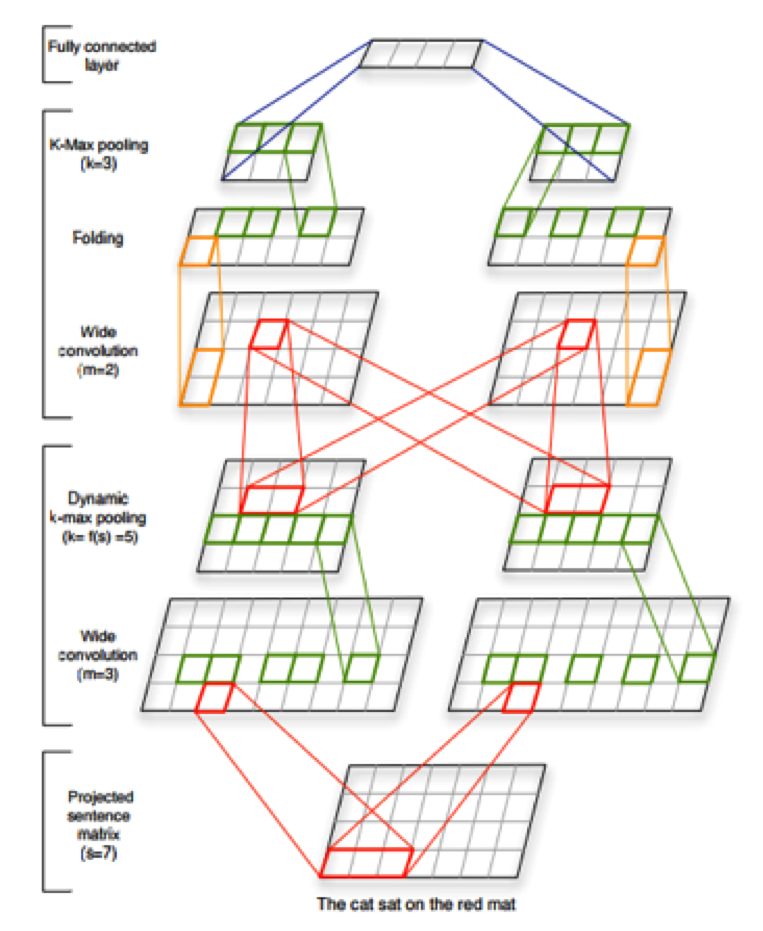
\includegraphics[height=4in, width=0.8\textwidth]{figs/DCNN.png}
	\caption{Dynamic Convulational Neural Network of \cite{kalchbrenner2014convolutional} (Source: \cite{kalchbrenner2014convolutional})}
	\label{fig:dcnn}
\end{figure}

\subsection{Recurrent Neural Networks with Long Short Term Memory (LSTM)}
Recurrent Neural Networks (RNNs) are a class of artificial neural networks used for modeling sequences.
RNNs are highly flexible in their use of context information as they can learn what part of the input sequence to store to memory and what parts to ignore. They also allow modeling of various regimes of sequence modeling as shown in Figure \ref{fig:rnn}. Please refer to \cite{graves2012supervised} for a comprehensive review of sequence modeling using RNN.

\begin{figure}
	\centering
	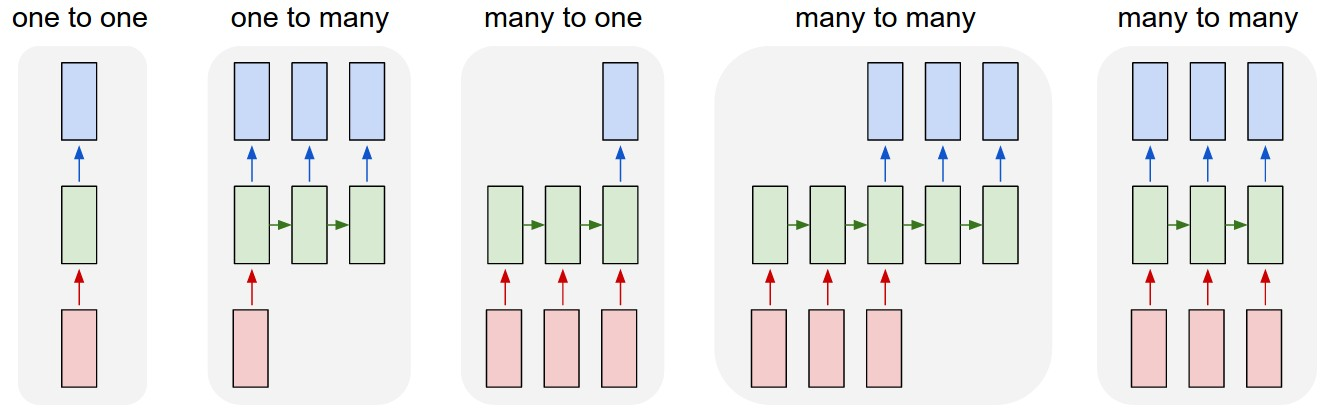
\includegraphics[width=\textwidth]{figs/rnn.jpeg}
	\caption{RNNs allow modeling of multiple types of input and output sequences (Source: \cite{karpathy-rnn})}
	\label{fig:rnn}
\end{figure}

One of the short comings of RNN is that it is very difficult to store information over long sequences because of problems due to vanishing and exploding gradients as explained in \cite{hochreiter2001gradient}.
{\it Long Short-Term Memory (LSTM)} \cite{hochreiter1997long} are designed to remedy this and store information over larger input sequences.
They achieve this using special ``memory cell'' units. 
Figure \ref{fig:lstm} shows the architecture of this cell which consists of an input gate, a forget gate, an output gate and a recurring cell state. 
Refer to \cite{colah} for a gentle introduction to LSTM and to \cite{graves2012supervised} for a more comprehensive review and applications.

\begin{figure}
	\centering
	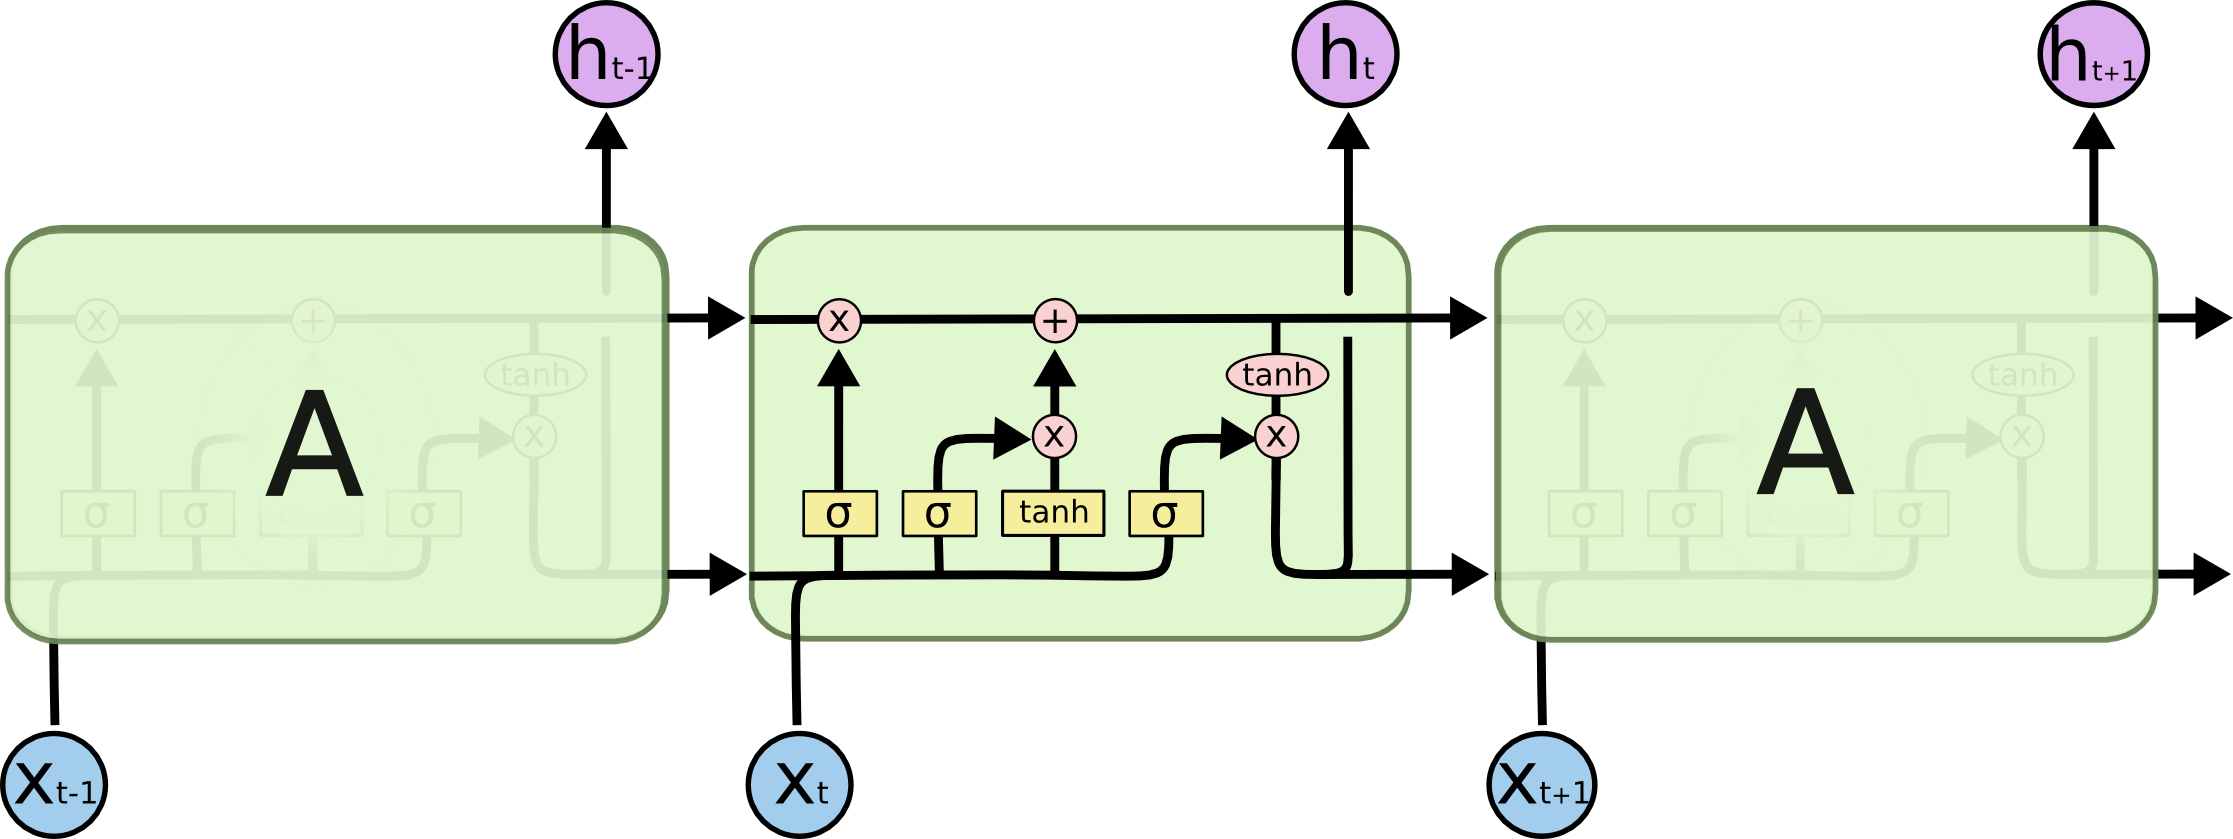
\includegraphics[width=\textwidth]{figs/LSTM.png}
	\caption{The repeating module of LSTM. $x_t$ is the input as time $t$ and $h_t$ is the output from the LSTM output gate at time $t$. The top horizontal line corresponds to the cell state and the bottom line corresponds to the hidden state (both of which are recurring states).
	(Source: \cite{colah})}
	\label{fig:lstm}
\end{figure}

\section{Twitter Sentiment Analysis using LSTM}
In this section we present LSTM models for sentiment analysis of twitter messages. We explored different architectures of LSTM networks which operate at word-level or character-level input. The basic architecture of the network is shown in Figure \ref{fig:mylstm}.
We explain the model architecture considering the character input.
Given a tweet as a sequence of characters $X=\{x_1, \ldots, x_{140}\}$, the task is to predict the sentiment of Tweet as being {\it positive} (1) or {\it negative} (0). Each $x_i$ is a one-hot encoding of either the character or the word. The LSTM models then take this one-hot encoding and convert them into either a {\it character embedding} or a {\it word embedding} depending on whether the input is characters or words. The embeddings can be randomly initialized and learned jointly with other model parameters.

The model consists of a bidirectional LSTM layer over this character input $X$. The hidden layer activations obtained from the forward and backward LSTM layer are averaged at {\it each} character which serves as the input to the {\it second layer} of LSTM. The second layer of LSTM takes as input this sequence of hidden layer outputs from first layer and encodes a representation of the tweet at the last element of the sequence (the hidden layer activation of the last LSTM unit). This output is then fed into a softmax layer which classifies the Tweet as being positive or negative.
The model is trained using categorical cross-entropy.

Note that it is possible to have multiple levels of granularity in predictions, like positive, ``netural" and negative, or even finer.
We restrict ourselves to two classes to be able to compare with the state of the art published results \cite{kalchbrenner2014convolutional}.

The same model can be used with either character input data or word input data. Note that when used with word input, it is common to initialize the models with pre-trained word embeddings \cite{mikolov2013distributed}. We explore multiple such initializations in our experiments.
For the character input model, the embeddings are always initialized randomly, since pre-trained character embeddings are not yet available.

We explored other variants of the model like have single-directional LSTM, having a single layer as opposed to multiple layers, using concatenation instead of averaging after first layer. We also tried an ensemble LSTM which takes both characters and words as separate inputs which are combined at the last stage by concatenation before feeding to the softmax. Unfortunately, none of these models gave good preliminary results and in the experiments we focused on just the model of Figure \ref{fig:mylstm} with either character or words as inputs.

\begin{figure}
	\centering
	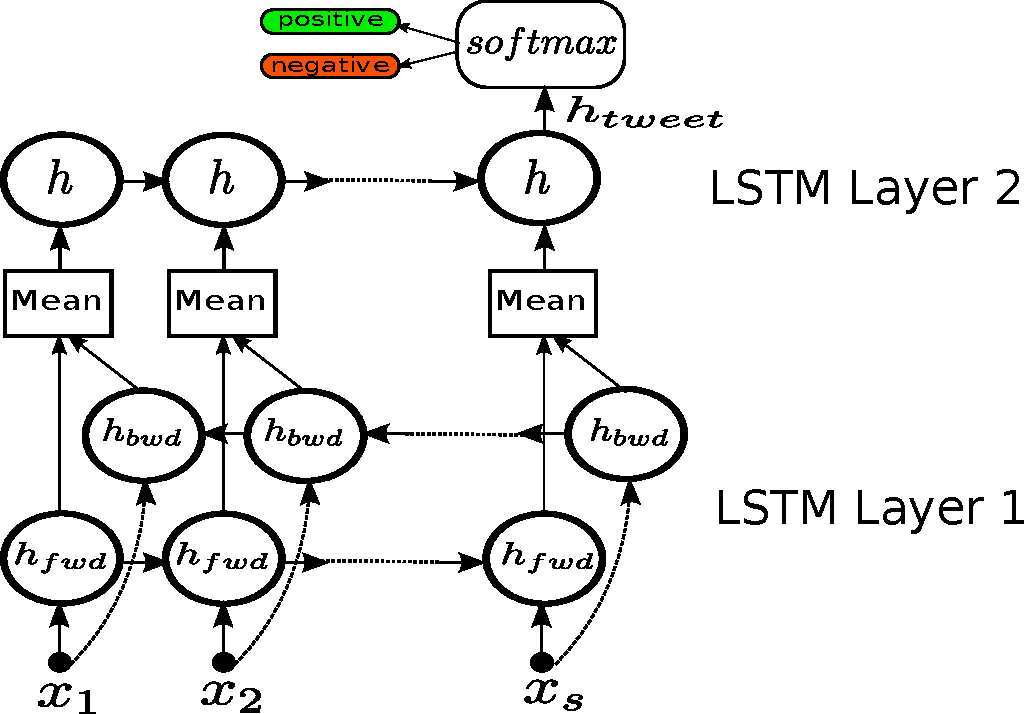
\includegraphics[width=\textwidth, height=3.6in]{figs/mylstm.pdf}
	\caption{The bi-directional LSTM model used for Twitter sentiment analysis. Each circular node represents an LSTM cell. The input to the model is the sequence $x$. }
	\label{fig:mylstm}
\end{figure}


\section{Results}

\subsection{Datasets}
We conduct our experiments on two datasets: the latest benchmark dataset for SemEval 2016 and the dataset provided by \cite{go2009twitter}. In the latter dataset, the training set consists of $1.6$ million weakly-supervised tweets collected during $2009$, and the test set is hand-labeled. In the experiments presented below, we first train our models on the Go dataset, then re-train the model parameters on the smaller, fully-supervised SemEval dataset.

\begin{table}[h!]
\centering
\caption{Data size and label distribution}
\begin{tabular}{|lllll|}
\hline
      & \multicolumn{2}{l}{Go et. al. (1.6M)} & \multicolumn{2}{l}{SemEval2016} \\
      & neg               & pos               & neg            & pos            \\
\hline
train & 800000            & 800000            & 781            & 2805           \\
dev   & -                 & -                 & 358            & 766            \\
test  & 177               & 182               & 286            & 886           \\
\hline
\end{tabular}
\label{table:corpus}
\end{table}

\subsection{Experiments}
We compare the performance of character-level models against word-level models. For the former, we compare across character sets (``utf8'' and ``ascii''), parameter initializations (``rnd'' and ``eye''), and embedding dimension sizes ($50$ and $200$). The vocabulary for the ``utf8'' setting consisted of $1949$ characters, and for ``ascii'' consisted of $93$ characters. We initialize model parameters randomly at all levels in the ``rnd'' setting whereas in the ``eye'' setting, we initialize the second-level LSTM cell and gate parameters using the identity matrix.

We compare word-level models under two settings: initializing the word embeddings using random vectors (``word/rnd'') and initialization using ``sentiment-specific'' word embeddings provided in \cite{tang2014learning} (``word/sswe'').

Our results are shown in Table ~\ref{table:results}. We train all models using the implementation of the Adam algorithm \cite{kingma2014adam} provided in Lasagne\footnote{\url{https://github.com/Lasagne/Lasagne}} and a learning rate set to $0.1$ \footnote{We retrained the ascii/rnd/200 on SemEval using AdaGrad and a learning rate of $0.01$ to achieve $84.13$; using Adam and $0.1$ learning rate, the result was $83.21$}. To learn word and character embeddings, we use a bidirectional LSTM with $256$ hidden units, followed by a mean pooling and a dropout layer ($p=0.5$), a second forward-directional LSTM (again with $256$ hidden units) and a final dropout layer ($p=0.6$). We obtain final predictions using the softmax function.

\begin{table}[h!]
\centering
\caption{Accuracy across LSTMs}
\begin{tabular}{|l|ll|}
\hline
              & 1.6M (acc)          & semeval (acc) \\
\hline
ascii/rnd/50  & 83.84          & 82.08            \\
ascii/rnd/200 & 82.45          & \textbf{84.13}   \\
ascii/eye/50  & 77.44          & 79.18   \\
utf8          & 81.34          & 82.34   \\
char-dcnn     & 75.0           & 81.3    \\
word/rnd      & 81.85          & 78.07   \\
word/sswe     & 83.24          & 79.27   \\
word/dcnn     & \textbf{87.4}\footnote{Reported in \cite{kalchbrenner2014convolutional}}           & 81.3    \\
\hline
\end{tabular}
\label{table:results}
\end{table}

The character-level models using the ``ascii'' character set outperformed the other models on the SemEval dataset. Due to the highly-productive nature of the Twitter ``lexicon'', users' predisposition toward using slang dialects, and the constraint of the $140$-character limit, it makes sense that word-level models underperform.

It is worth noting that the ``utf8'' model performed comparably despite having a much larger vocabulary size. It is not suprising that the ``utf8'' model performed worse than the ``ascii'' model, as the test data consisted of only English tweets; however, since the ``utf8'' model is implicitly multi-lingual, our results suggest that the same model may perform well across multiple languages. We leave such experiments for future work.

As Table ~\ref{table:results} shows, \cite{kalchbrenner2014convolutional} outperform our character LSTM on the Go dataset. However, the results presented for our character and word-level models achieve competitive performance on the Go dataset without tuning hyperparameters such as learning rate and network width. 

\subsection{Qualitative Analysis}
Figure ~\ref{fig:cool} shows the effect of character repetition on model confidence over the course of the sequence, where confidence is computed using the softmax function:

$$P(y = j|\mathbf{x}) = \frac{e^{\mathbf{x}^T \mathbf{w}_j}}{\sum_{k=1}^{K} e^{\mathbf{x}^T \mathbf{w}_k}}$$

In our experiments, we had $K = 2$ corresponding to binary classification between ``positive'' and ``negative'' tweets. Sequences ending in periods (``cool.'', ``coool.'') ended up with less-confident scores than tweets not ending in periods. Repeated exclamation points don't increase the model's confidence in the ``positive'' label as much as might be expected. 

\begin{figure}[h!]
\begin{center}
%\framebox[4.0in]{$\;$}
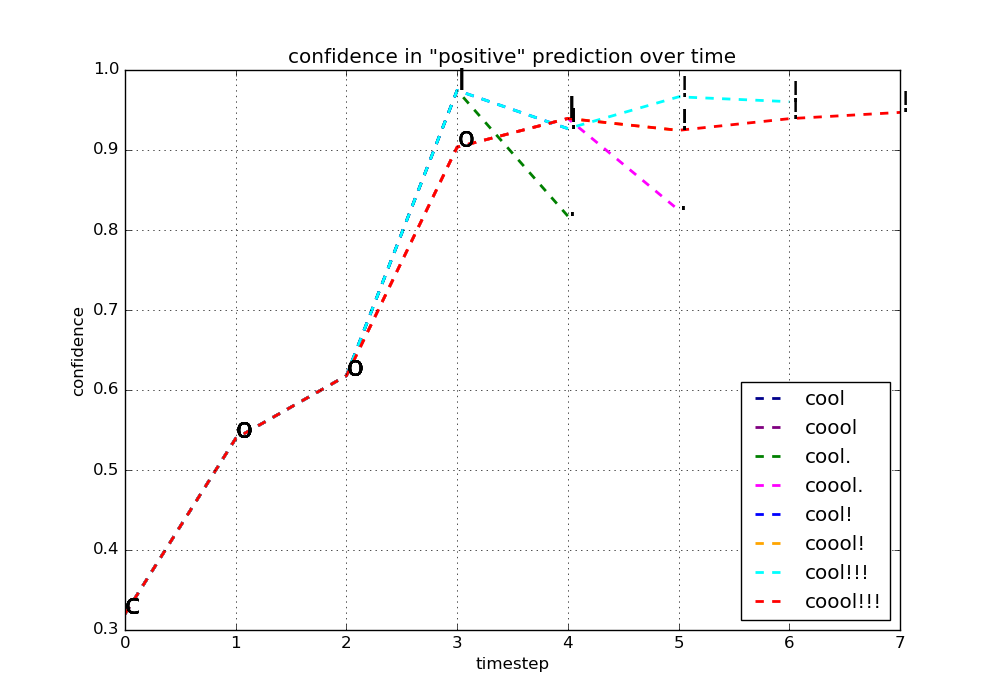
\includegraphics[width=0.95\textwidth]{figs/cool}
%\fbox{\rule[-.5cm]{0cm}{4cm} \rule[-.5cm]{4cm}{0cm}}
\end{center}
\caption{Comparison of model confidence for different forms of the word ``cool''}
\label{fig:cool}
\end{figure}

Figure ~\ref{fig:puppies} shows that the character-level model learns word meaning at a lexical level: the predictions for ``I love puppies'' and ``I hate puppies'' diverges sharply after the model has finished reading ``lov'' (``love'') and ``hat'' (``hate'').

\begin{figure}[h!]

\begin{center}
%\framebox[4.0in]{$\;$}
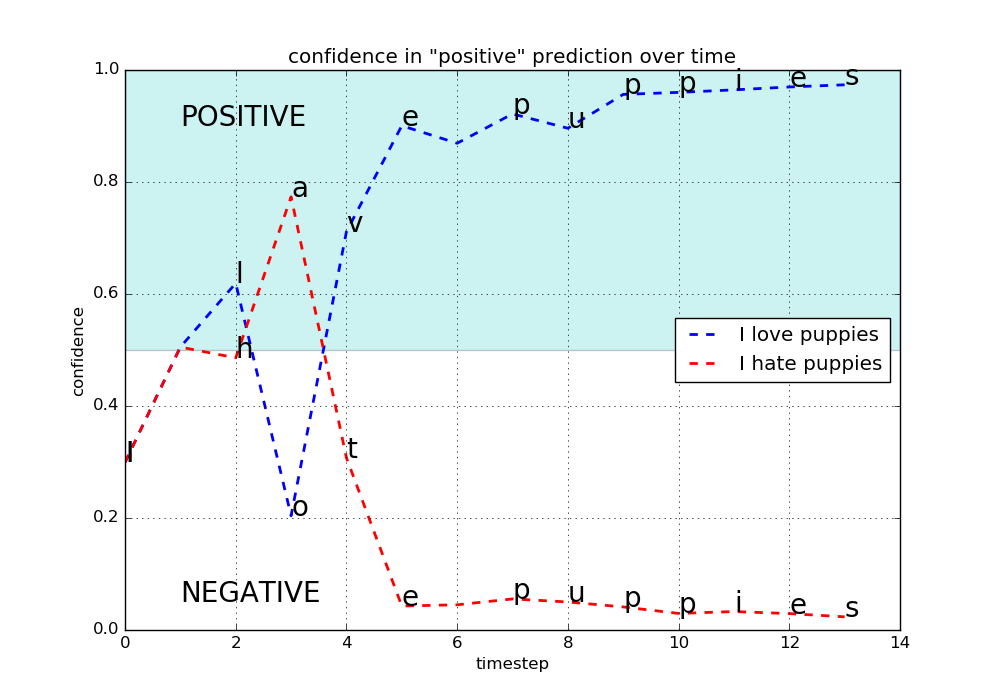
\includegraphics[width=0.95\textwidth]{figs/puppies}
%\fbox{\rule[-.5cm]{0cm}{4cm} \rule[-.5cm]{4cm}{0cm}}
\end{center}
\caption{Comparison of model confidence for ``I love puppies'' vs. ``I hate puppies''}
\label{fig:puppies}
\end{figure}

Figure ~\ref{fig:dentist} provides further evidence that character-level models can reason about lexical semantics in an intuitive fashion. We compare confidence contours across four tweets from the Go test set. The ground truth labels for the first two tweets are both ``negative'', and for the second two are both ``positive''. In the first two, the model finds strong evidence for a ``negative'' prediction before reaching the word ``dentist'', and correctly predicts that both tweets are ``negative''. In the second two, the word ``dentist'' results in an increase in the model's confidence in a ``negative'' prediction; however, the words ``enjoyable'' and ``:)'' cause the model's confidence to decrease in the ``positive'' direction. 

\begin{figure}[h!]

\begin{center}
%\framebox[4.0in]{$\;$}
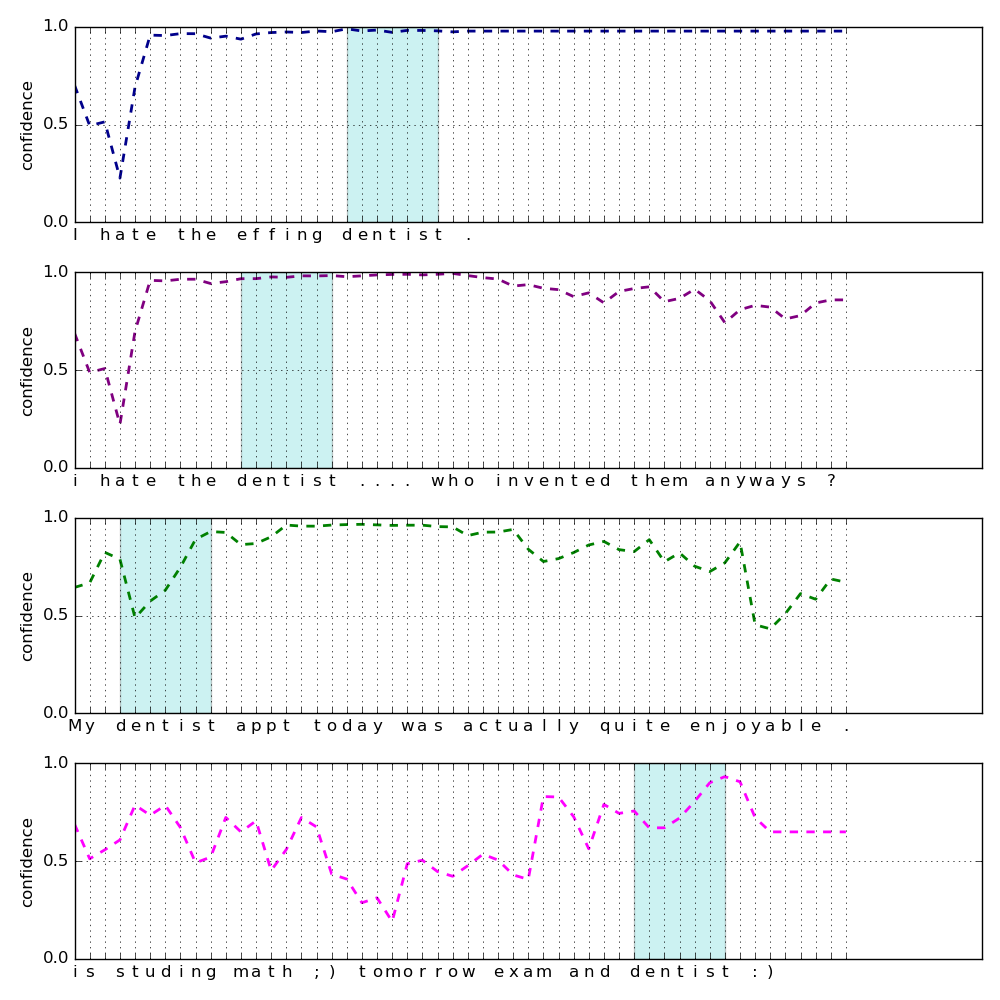
\includegraphics[width=0.95\textwidth]{figs/dentist}
%\fbox{\rule[-.5cm]{0cm}{4cm} \rule[-.5cm]{4cm}{0cm}}
\end{center}
\caption{Confidence in ``negative'' prediction over time across four tweets}
\label{fig:dentist}
\end{figure}

Table ~\ref{table:word-sim} shows words alongside their nearest neighbors computed using the character embeddings learned by our model. As desired, othographic variations of the same word ``type'' are close together in the embedding space. 

\begin{table}[h!]
\begin{center}
\begin{tabular}{|l|l|}
\hline
woohoo &    wooohoo woohooo wooohooo woohoooo wooooo whoooo woooo whoohoo \\
wohooo\
woww &   wowww wow whack vwv waw vry cow werk woke \\
xoxo &    xox xoxox zoo xxoo vox xoxoxo zoe xxo twix \\
thanks &    thankss thanku yanks thankx hanks thankz thanksss tanks thanx \\
sorry &    sorrry srry scary sowwy sorryyy scared sory scarred errrr \\
sucks &   sucky suckss yucky eurgh ouchy suckish fucks ouchh jerks \\
twitter &    twiter twiiter tinytwitter twitterr quicker txting \\
granddaughter & ktbeeper twitting \\
tweet  &  tweeet tweep tweety tweets textt theee seee outer peace \\
\hline
\end{tabular}
\end{center}
\caption{Words and their nearest neighbors}
\label{table:word-sim}
\end{table}

\section{Conclusion}
In this paper, we show promising empirical evidence that character-level models perform well for sentiment analysis on tweets, which are ``noisy'', in that users think of millions of new words and spellings of words every day, and ``brief'', in that they are constrained to $140$ characters. This type of text data is becoming an important research focus in the field of NLP, as data is often cheap to collect in high volume and can provide important insight into society-wide trends. Though the experiments in this paper focus on sentiment classification, we believe our results provide a basis for future work on character-level modeling for a variety of other NLP tasks.

\bibliography{paper}
\bibliographystyle{plain}
%% References follow the acknowledgments. Use unnumbered third level heading for
%% the references. Any choice of citation style is acceptable as long as you are
%% consistent. It is permissible to reduce the font size to `small' (9-point) 
%% when listing the references. {\bf Remember that this year you can use
%% a ninth page as long as it contains \emph{only} cited references.}

%% \small{
%% [1] Alexander, J.A. \& Mozer, M.C. (1995) Template-based algorithms
%% for connectionist rule extraction. In G. Tesauro, D. S. Touretzky
%% and T.K. Leen (eds.), {\it Advances in Neural Information Processing
%% Systems 7}, pp. 609-616. Cambridge, MA: MIT Press.

%% [2] Bower, J.M. \& Beeman, D. (1995) {\it The Book of GENESIS: Exploring
%% Realistic Neural Models with the GEneral NEural SImulation System.}
%% New York: TELOS/Springer-Verlag.

%% [3] Hasselmo, M.E., Schnell, E. \& Barkai, E. (1995) Dynamics of learning
%% and recall at excitatory recurrent synapses and cholinergic modulation
%% in rat hippocampal region CA3. {\it Journal of Neuroscience}
%% {\bf 15}(7):5249-5262.
%% }

\end{document}
